\documentclass[12pt]{article}

\usepackage{sbc-template}

\usepackage{graphicx,url}

\usepackage[brazil]{babel}   
\usepackage[utf8]{inputenc}  
\usepackage[table,xcdraw]{xcolor}
\usepackage{pdfpages}
     
\sloppy

\title{Comparação de técnicas de aprendizado de máquina utilizando o WEKA\\ }

\author{Amilton Fontoura de Camargo Junior\inst{1}, Kauane Larisse de Oliveira Benitis\inst{1}}


\address{Curso de Engenharia de Computação -- Universidade Tecnológica Federal do Paraná (UTFPR)\\
  CEP -- 86.300-000 -- Cornélio Procópio -- PR -- Brasil
  \email{amiltonjunior2007@gmail.com,
  kauane@alunos.utfpr.edu.br}
}

\begin{document} 

\maketitle
\begin{abstract}
This paper presents a comparison study of supervised and unsupervised machine learning techniques using 10 different data sets in the open source WEKA tool for data mining and a new machine learning proposal.
\end{abstract}
     
\begin{resumo}
Esse trabalho apresenta um estudo de comparação de técnicas de aprendizado de máquinas supervisionado e não supervisionado, utilizando 10 diferentes conjuntos de dados na ferramenta WEKA de código aberto, para mineiração de dados e uma nova proposta de aprendizado de máquina.
\end{resumo}


\section{Introdução} \label{sec:intro}

	Inteligência artificial é um termo abrangente que engloba o Aprendizado de Máquina (AM), que é o conjunto de técnicas e ferramentas que permitem que o computador "pense" criando algoritmos matemáticos baseados em dados acumulados. Também sob esse termo genérico está o Aprendizado Profundo (AP), um subconjunto do aprendizado de máquina que utiliza modelos de redes neurais para executar tarefas como reconhecimento de imagem e processamento de linguagem.
	
	A inteligência artificial propicia diversas melhorias em áreas distintas. Ao medir a biometria no esporte, os dados podem ajudar a avaliar de que modo o tempo de atividade dos atletas afeta a probabilidade de lesões. Ajudam os agricultores a saber quando regar as plantações para obter colheitas excelentes, permitem que os meteorologistas calculem o degelo \cite{database}. Cidades inteligentes utilizam dados para o gerenciamento de energia, profissionais de saúde recorrem à inteligência artificial para detectar doenças, realizar sequenciamento genômico e acompanhar tratamentos.


\section{Técnicas e Ferramentas Utilizadas} \label{sec:tecnicas}

\subsection{Introdução} \label{sec:introducao}

O estudo das técnicas de aprendizado de máquina foi dividido em 5 partes. A primeira parte consistiu em:

\begin{itemize}
	\item Selecionar 10 conjuntos de dados;
	\item Fazer uma tabela com as informações dos conjuntos de dados;
	\item Descrever sucintamente o conjunto de dados;
	\item Construir um programa que realizava a divisão do conjunto de dados;
\end{itemize}

A segunda parte do estudo foi para realizar experimentos e analisar resultados aplicando as técnicas de aprendizado supervisionado, vistos na sequencia do trabalho.

A aplicação da técnica não supervisionada deu-se na terceira etapa, onde foi utilizado o algoritmo k-means.

A proposta da quarta parte do estudo foi descrever uma nova estratégia de aprendizado, de forma a selecionar amostras mais representativas e informativas ao processo de aprendizado do classificador.

\subsection{O ambiente WEKA} \label{sec:ambienteweka}

    O WEKA é um software de código aberto implementado por um grupo de aprendizado de máquina da Universidade de Waikato, que atualmente fornece algoritmos que podem ser facilmente aplicados a grandes conjuntos de dados. WEKA implementa várias classificações de aprendizado de máquina, algoritmos de regressão e agrupamento, juntamente com uma série de ferramentas de visualização. Hoje \cite{cancer} em dia, é aceito como um dos ambiente mais poderosos e adequados para a mineração de dados. Sua interface principal possibilita que o usuário escolha uma das quatro aplicações disponíveis, isto é, o Explorador, o Experimentador, o Fluxo de Conhecimento e uma Interface de Linha de Comando.
    
    Ao longo desse estudo, todos os dados analisados estavam no formato ARFF (Arquivo de Relação Formato de Atributo), que é o formato  de arquivo que o WEKA utiliza. O conjunto de dados escolhidos para o desenvolvimento desse estudo deu-se de maneira aleatória, porém variando entre os conjuntos o número de amostras, classes a atributos.
    
\subsection{Técnicas} \label{sec:tec}

    A comparação realizada e apresentada nesse trabalho engloba seis tipos de técnicas de aprendizagem, descritas a seguir.
    
\subsection{Divisão} \label{sec:split}

    A divisão consistiu em separar o conjunto de dados de maneira a obter uma parte para teste e outra parte para treinamento, podendo ser escolhida a porcentagem para cada fim.
    
\begin{figure}[h]
\centering
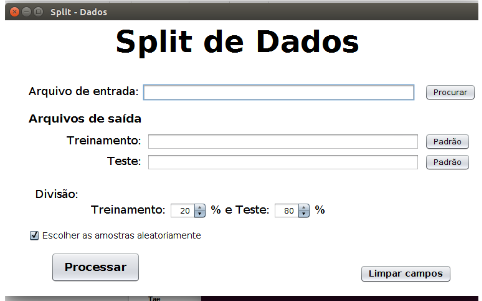
\includegraphics[width=.68\textwidth]{split.png}
\caption{Interface do programa para divisão do conjunto de dados}
\label{fig:split}
\end{figure}
        
    A interface do programa utilizado para realizar a divisão do conjunto pode ser visualizada na Figura \ref{fig:split}. O conjuntos selecionados na divisão, eram particionados em doid subconjuntos, um para teste e outro para treinamento, ambos eram salvos na mesmo local do conjunto original como pode ser visto na figura \ref{fig:splitt}.
        
\begin{figure}[h]
\centering
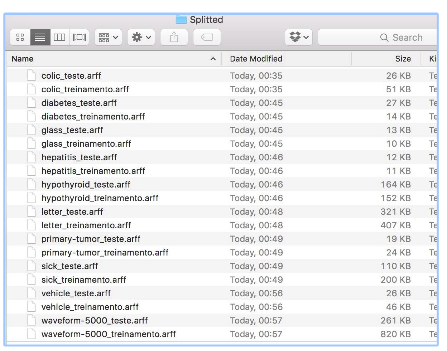
\includegraphics[width=.68\textwidth]{splitt.png}
\caption{Conjuntos de Treinamento e Testes}
\label{fig:splitt}
\end{figure}
    

\subsubsection{Validação Cruzada} \label{sec:cv10}

    A validação cruzada é um processo de aprendizagem supervisionada em mineração de dados onde o conjunto é dividido em duas partes, sendo uma para teste e outra para treinamento.
    
    Numa primeira etapa um algoritmo de indução de conhecimento é aplcado à base de treinamento. Na segunda etapa o modelo obtido é aplicado ao fragmento da base de dados que foi dividido como teste. Como a base de testes é previamente rotulada torna-se possível medir  a taxa de acerto do modelo.
    

\subsubsection{Naive Bayes} \label{sec:nb}

    Naive Bayes é um classificador bayesiano e produz regras probabilísticas. Quando um novo item de dados é apresentado, categoriza-o, apresentando um porcentagem de probabilidade em direção as possíveis categorias de classes \cite{cancer}. A classificação é realizado quando a regra de Bayes bem conhecida é aplicada em cada atribbut do modelo e a probabilidade sobre uma variável de classe independente é calculado.

\subsubsection{Árvore de Decisão - J48} \label{sec:j48}

    Entre as várias técnicas de aprendizado de máquina, a árvore de decisão pode ser caracterizada como  uma das mais usadas. Representa o mapeamento dos atributos e consiste em nó que ligam duas ou mais subárvores. O nó calcula um resultado específico baseado no valor da instância e cada possível resultado está ligado com uma das subárvores. O algoritmo J48, uma implementação do C4.5 versão 8, é um método eficiente para estimação e classificação de dados fuzzy \cite{cancer}.
    
\subsubsection{Rede Neural - MultiLayer Perceptron} \label{sec:mlp}

    A Rede Neural é um sistema adaptativo que muda sua estrutura baseado em informações externas e internas através de uma rede durante uma fase de aprendizado inicial. Em termos mais práticos, as redes neurais são estatísticas não lineares de modelagem de dados. Podem ser usadas em modelos complexos de relacionamentos entre entradas e saídas ou para encontrar padrões de dados \cite{cancer}.

\subsubsection{k-Vizinhos Mais Próximos - IBk} \label{sec:ibk}

    Uma das formas mais simples de algoritmos de classificação é a implementação dos Vizinhos Mais Próximos. Tais esquemas de aprendizado são delineados como algorítimos de aprendizagem estatística e são gerados simplesmente por dados armazenados. Para que a classificação seja uma métrica de distância é escolhido um dado qualquer e comparado com itens de dados "memorizados" totalmente prontos \cite{rezende2003sistemas}. O novo item é atribuído à classe que é mais comum entre seus k-vizinhos mais próximos classificados. O número de vizinhos mais próximos(k) podem ser atribuídos de maneira manual ou determinados automaticamente usando validação cruzada.

\subsubsection{kMeans} \label{sec:kmean}

    O k-means é um algoritmo de mineração de dados não supervisionado, ou seja, fornece uma classificação de informações de acordo com os próprios dados \cite{database}. Está classificação é baseada em análise e comparações entre valores numéricos dos dados. Desta maneira, o algoritmo automaticamente vai fornecer uma classificação sem a necessidade de nenhum supervisão humana, isto é, sem nenhuma pré-classificação já existente.
    
    O algoritmo vai analisar todos os dados e criar classificações, de modo que uma classe(cluster) será indicada para  dizer quais linhas linhas pertencem a esta classe \cite{smoke}. Conforme a quantidade de classes desejadas, este número deve ser passado para o algoritmo.
    
\subsection{Conjunto de Dados} \label{sec:dataset}

    Foram escolhidos 10 conjunto de dados de maneira aleatória, procurando selecionar conjuntos em que diversificassem o número de amostras, números de classes e números de atributos.
    
    O conjunto de dados selecionados pode ser visualizado na tabela \ref{tabelaConjuntoDados}, juntamente com suas características utilizadas para aplicar as técnicas de aprendizado de máquina.

\begin{table}[h]

	\centering
	\caption{Conjunto de Dados}
	\label{tabelaConjuntoDados}
	\begin{tabular}{lccccc}
		\hline
		Nome do Conjunto & Número de Amostras & Número de Classes & Número de Atributos \\ \hline
		Colic  & 63983    & 368  & 23    \\ \hline
		Dermatology  & 32417    & 366  & 35    \\ \hline
		Diabetes  & 37419    & 768  & 9    \\ \hline
		Glass  & 17823    & 214  & 10    \\ \hline
		Hepatitis  & 17135    & 155  & 20    \\ \hline
		Hypothyroid  & 310897    & 3772  & 30    \\ \hline
		Iris  & 7486    & 150  & 4    \\ \hline
		Primary Tumor  & 34090    & 339  & 18    \\ \hline
		Vehicle  & 63838    & 4  & 18    \\ \hline
		Tae  & 4120    & 151  & 6    \\ \hline
	\end{tabular}
\end{table}

\subsubsection{Descrição dos Conjunto de Dados} \label{sec:descricaodataset}

A seguir serão descritos de maneira breve cada conjunto de dados selecionado para realizar o estudo atual.

\subsubsubsection{Colic} \label{sec:colic}

Esse conjunto é uma base de dados de cólica de cavalo, onde foram separados 300 instâncias para treinamento e 68 para testes. Apresenta tipos de dados contínuos, discretos e nominais e 28 atributos.

\subsubsubsection{Dermatology} \label{sec:derma}

Este banco de dados contém 34 atributos, dos quais 33 são valores lineares  e 1 nominal. Todos eles compartilham características de eristemas (clínicas e histapatológicas).

\subsubsubsection{Diabetes} \label{sec:diabetes}

Base de dados de diabetes onde foi usado 576 intâcias para treinamento e 192 para testes por meio do algoritmo ADAP para servir de variável diagnóstica de pacientes que apresentam sinais de diabetes.

\subsubsubsection{Glass} \label{sec:glass}

Glass é uma base de dados de 214 intanciâs onde foi empregado o algoritmo do vizinho mais próximo e análise discriminante para determinar se o vidro era do tipo flutuante, onde classifica-se por exemplo se o vidro em questão pertence a uma janela de casa ou de carro.

\subsubsubsection{Hepatitis} \label{sec:hepatitis}

Este banco de dados contem características apresentadas em portadores de hepatite como método computarizado para realizar diagnóstido de hepatite. As informações apresentadas nas 155 instâncias estão relacionadas com 32 indivíduos que já entraram em óbito e 123 vivos.

\subsubsubsection{Hypothyroid} \label{sec:hypo}

Base de dados compostas por 3272 instâncias cujos atributos permitem identificar a hipotireóide primária, compensada, negativo e hipotireóide conforme os atributos.

\subsubsubsection{Iris} \label{sec:iris}

O conjunto de dados contem 150 instancias onde 3 classes de 50 instancias se refere a um tipo da planta Iris.

\subsubsubsection{Primary Tumor} \label{sec:tumor}

Primary Tumor contem 339 instâncias e 18 atributos onde um dos atributos é a classe de localização de tumor.

\subsubsubsection{Vehicle} \label{sec:vehicle}

Conjunto de dados que usa um conjunto de recursos da silhueta para classificar conforme os quatro tipos de veículos do banco.

\subsubsubsection{Tae} \label{sec:tae}

Base de dados para avaliação de assistente de ensino onde os dados consistem em avaliações de desempenho de ensino em três semestres regulares e dois meses de verão caracterizados em baixo, medio e alto para formar a variável de classe

\section{Análise e Resultados} \label{sec:analise}

Aqui serão apresentados os resultados obtidos nos experimentos realizados com o WEKA, mostrando o custo de cada conjunto de dados, acurácia de cada conjunto de dados, média e desvio padrão de custo de cada técnica por conjunto, média e desvio padrão de custo de conjunto considerando todas as técnicas, acurácia de cada técnicas por conjunto, acurácia de conjunto considerando todas as técnicas.

Esse dados serão mostrados no trabalho por  meio de gráficos e tabelas no decorrer do trabalho, assim como uma análise sobre os mesmos.


\begin{table}[h]

	\centering
	\caption{Média e Desvio Padrão dos Conjuntos de Dados}
	\label{tabelaMediaDP}
	\begin{tabular}{lcccccc}
		\hline
		Nome do Conjunto & Média de Acurácia & DP de Acurácia & Média de Custo & DP de Custo \\ \hline
		Colic  & 79,11 & 15,53 & 0,71 & 1,94 \\ \hline
		Dermatology  & 72,35 & 34,63 & 2,97 & 8,32  \\ \hline
		Diabetes  & 77,55 & 14,52 & 0,13 & 0,20 \\ \hline
		Glass  & 81,09 & 27,11 & 0,05 & 0,13 \\ \hline
		Hepatitis  & 85,73 & 8,86 & 0,05 & 0,11 \\ \hline
		Hypothyroid  & 96,74 & 3,58 & 4,66 & 7,78 \\ \hline
		Iris  & 73,67 & 33,43 & 0,01 & 0,03 \\ \hline
		Primary Tumor  & 50,33 & 31,95 & 0,96 & 1,72 \\ \hline
		Vehicle  & 58,81 & 32,03 & 0,43 & 0,73 \\ \hline
		Tae  & 58,39 & 26,36 & 0,02 & 0,03 \\ \hline
	\end{tabular}
\end{table}

Na tabela \ref{tabelaMediaDP} pode-se observar que o conjunto Hypothyroid obteve melhor média de acurácia e menor desvio padrão, no entanto, também foi o que apresentou maior custo. Também na tabela \ref{tabelaMediaDP} verificou-se que a base dados Primary Tumor teve a menor média de acurácia, assim como não houve média inferior à 50\% em nenhum outro conjunto.

\subsection{Acurácia das técnicas} \label{sec:acuracia}

Os resultados das acurácias obtidos de cada técnica utilizada no estudo mostrados na tabela \ref{tabelaAcuraciaConjuntoDados} estão apresentado a seguir.

\begin{table}[h]
	\centering
	\caption{Acurácia }	
	\label{tabelaAcuraciaConjuntoDados}
	\begin{tabular}{lccccccccc}
		\hline
		Conjunto & CV & NB & J48 & MLP & IBk1 & IBk2 & kMeans1 & kMeans2 \\ \hline
		Colic  & 63,04 & 77.99 & 85,33 &80,43 & 63,04 & 63,04 & 100,00 & 100,00 \\ \hline
		Dermatology & 30,60 & 97,27 & 93,99 & 96,17 & 30,60 & 30,60 & 99,80 & 99,80\\ \hline
		Diabetes & 65,10 & 76,30 & 73,83 & 75,39 & 65,10 & 65,10 & 99,80 & 99,80 \\ \hline
		Glass & 35,51 & 48,60 & 66,82 & 67,76 & 35,51 & 35,51 & 99,50 & 99,50 \\ \hline
		Hepatitis & 79,35& 84,52 & 83,87 & 80,00 & 79,35 & 79,35 & 99,70 & 99,70 \\ \hline
		Hypothyroid  & 92,29 & 95,28 & 99,58 & 94,17 & 92,29 & 92,29 & 100,00 & 100 \\ \hline
		Iris & 33,33 & 96,00 & 96,00 & 97,33 & 33,33 & 33,33 & 100,00 & 100,00 \\ \hline
		Primary Tumor & 24,78 & 50,15 & 39,82 & 38,35 & 24,78 & 24,78 & 100,00 & 100,00\\ \hline
		Vehicle & 25,65 & 44,80 & 72,46 &81,68 & 25,65 & 25,65 & 94,60 & 100,00 \\ \hline
		Tae & 34,44 & 54,30 & 59,60 & 54,30 & 34,44 & 34,44 & 97,80 & 97,80 \\ \hline
		\textbf{Média} & 48,41 & 72,52 & 77,13 & 76,56 & 48,41 & 48,41 & 99,12 & 99.66\\ \hline
		\textbf{Desvio Padrão} & 24,40 & 21,19 & 18,54 & 18,90 & 24,40 & 24,40 & 1,72 & 0,68 \\ \hline
	\end{tabular}
\end{table}

\begin{figure}[!h]
\centering
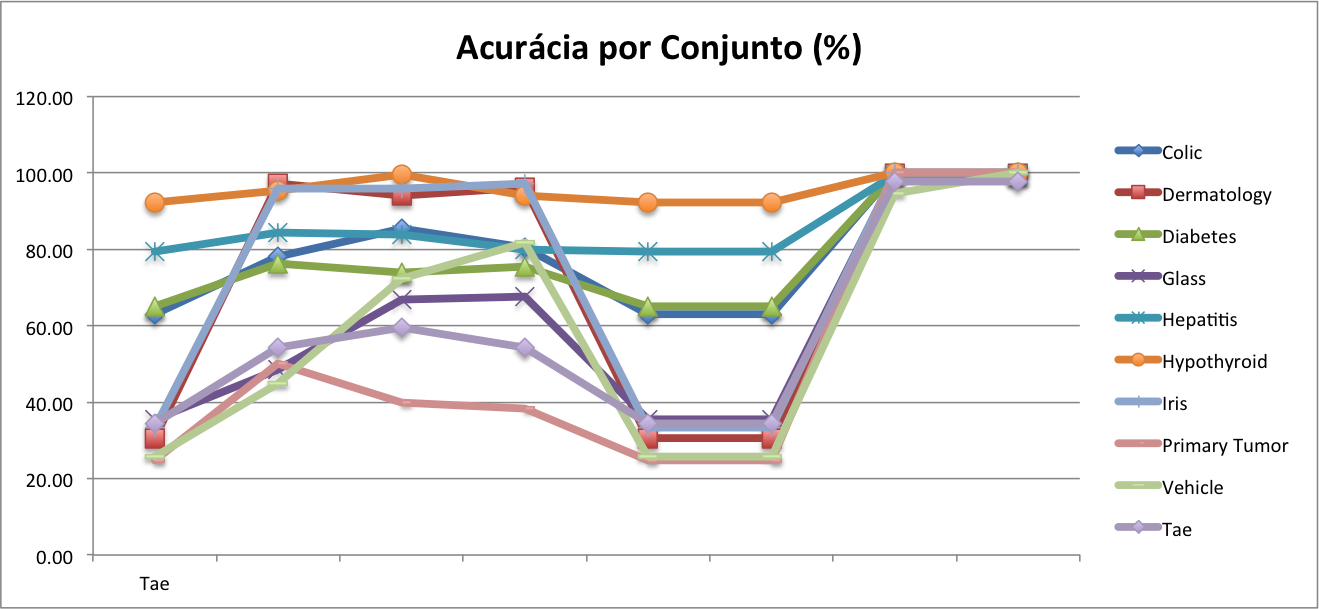
\includegraphics[width=.68\textwidth]{AcuraciaConjunto.png}
\caption{Gráfico da Acurácia de Cada Conjunto de Dados}
\label{fig:acuraciaconjunto}
\end{figure}

\begin{figure}[!h]
\centering
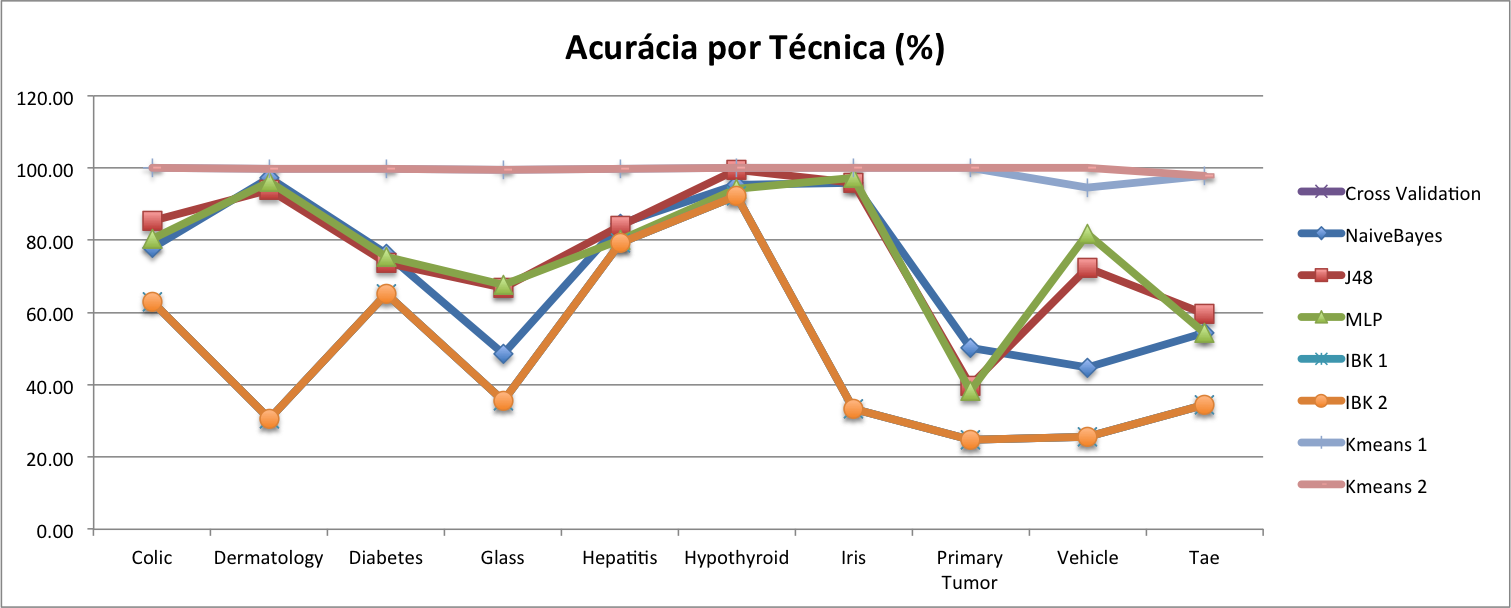
\includegraphics[width=.68\textwidth]{AcuraciaTecnica.png}
\caption{Gráfico da Acurácia das Técnicas de Aprendizado}
\label{fig:acuraciatecnica}
\end{figure}

A tabela \ref{tabelaAcuraciaConjuntoDados} juntamente com as figuras  \ref{fig:acuraciaconjunto} e figura \ref{fig:acuraciatecnica} mostraram que independente da técnica de aprendizado de máquina utilizada, a base de dados Hypothyroid foi a que apresentou os melhores valores. Das técnicas supervisionadas, as que mostraram melhor acurácia foram a J48 e a MultiLayer Perceptron, e, as que demonstraram menor eficiência no aprendizado foram a Cross Validation e IBk.

\subsection{Custos das técnicas} \label{sec:custo}

Os custos obtidos de cada técnica utilizada no estudo mostrados na tabela \ref{tabelaCustoConjuntoDados} estão dispostos na sequência.

\begin{table}[h]
	\centering
	\caption{Custo }
	\label{tabelaCustoConjuntoDados}
	\begin{tabular}{lccccccccc}
		\hline
		Conjunto & CV & NB & J48 & MLP & IBk1 & IBk2 & kMeans1 & kMeans2 \\ \hline
		Colic  & 0,00 & 0,01 & 0,01 & 5,51 & 0,00 & 0,00 & 0,11 & 0,07 \\ \hline
		Dermatology & 0,00 & 0,00 & 0,00 & 23,56 & 0,00 & 0,00 & 0,11 & 0,11 \\ \hline
		Diabetes & 0,00 & 0,00 & 0,02 & 0,57 & 0,00 & 0,00 & 0,27 & 0,15 \\ \hline
		Glass & 0,00 & 0,00 & 0,01 & 0,38 & 0,00 & 0,00 & 0,01 & 0,02 \\ \hline
		Hepatitis & 0,00 & 0,00 & 0,00 & 0,32 & 0,00 & 0,00 & 0,01 & 0,02 \\ \hline
		Hypothyroid  & 0,00 & 0,01 & 0,02 & 21,92 & 0,00 & 0,00 & 7,78 & 7,51 \\ \hline
		Iris & 0,00 & 0,00 & 0,00 & 0,09 & 0,00 & 0,00 & 0,01 & 0,01 \\ \hline
		Primary Tumor & 0,00 & 0,00 & 3,74 & 3,76 & 0,00 & 0,00 & 0,11 & 0,06 \\ \hline
		Vehicle & 0,00 & 0,00 & 0,10 & 2,12 & 0,00 & 0,00 & 0,60 & 0,62 \\ \hline
		Tae & 0,00 & 0,00 & 0,00 & 0,10 & 0,00 & 0,00 & 0,10 & 0,10 \\ \hline
		\textbf{Média} & 0,00 & 0,00 & 0,39 & 5,83 & 0,00 & 0,00 & 0,91 & 0,86 \\ \hline
		\textbf{Desvio Padrão} & 0,00 & 0,00 & 1,18 & 9,10 & 0,00 & 0,00 & 2,42 & 2,34 \\ \hline
	\end{tabular}
\end{table}


\begin{figure}[!h]
\centering
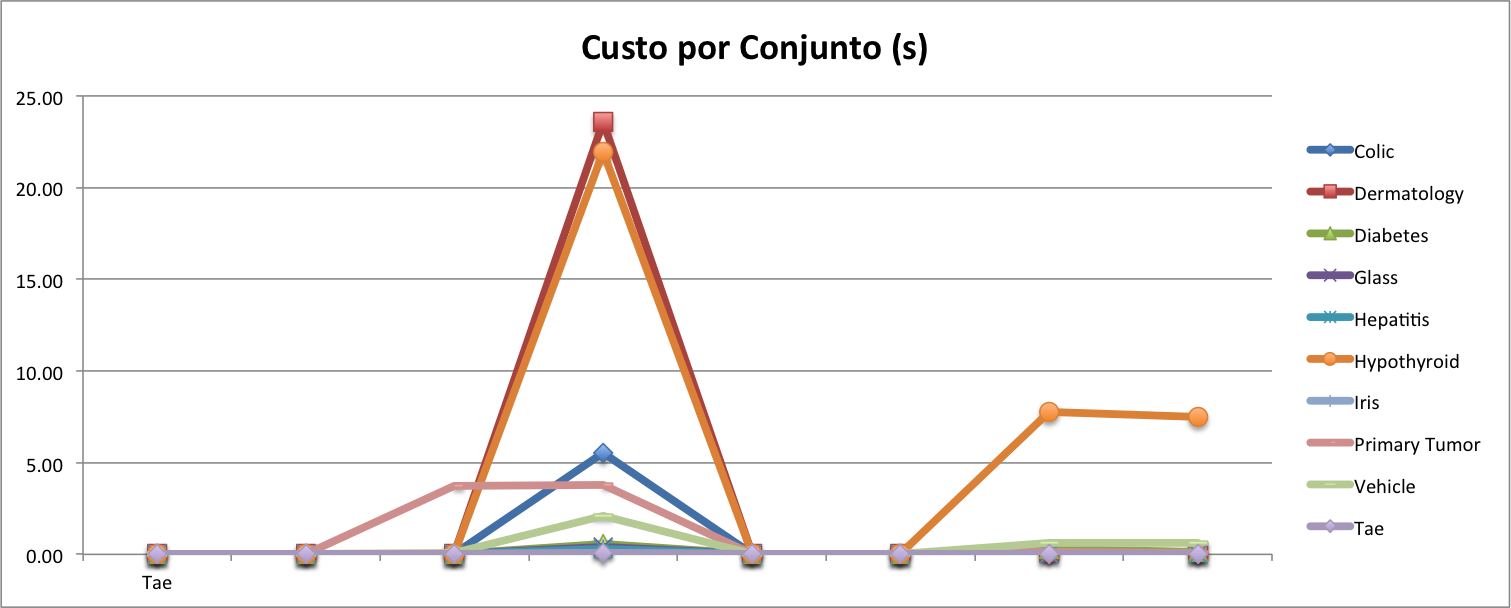
\includegraphics[width=.68\textwidth]{CustoConjunto.png}
\caption{Gráfico do Custo de Cada Conjunto de Dados}
\label{fig:custoconjunto}
\end{figure}

\begin{figure}[!h]
\centering
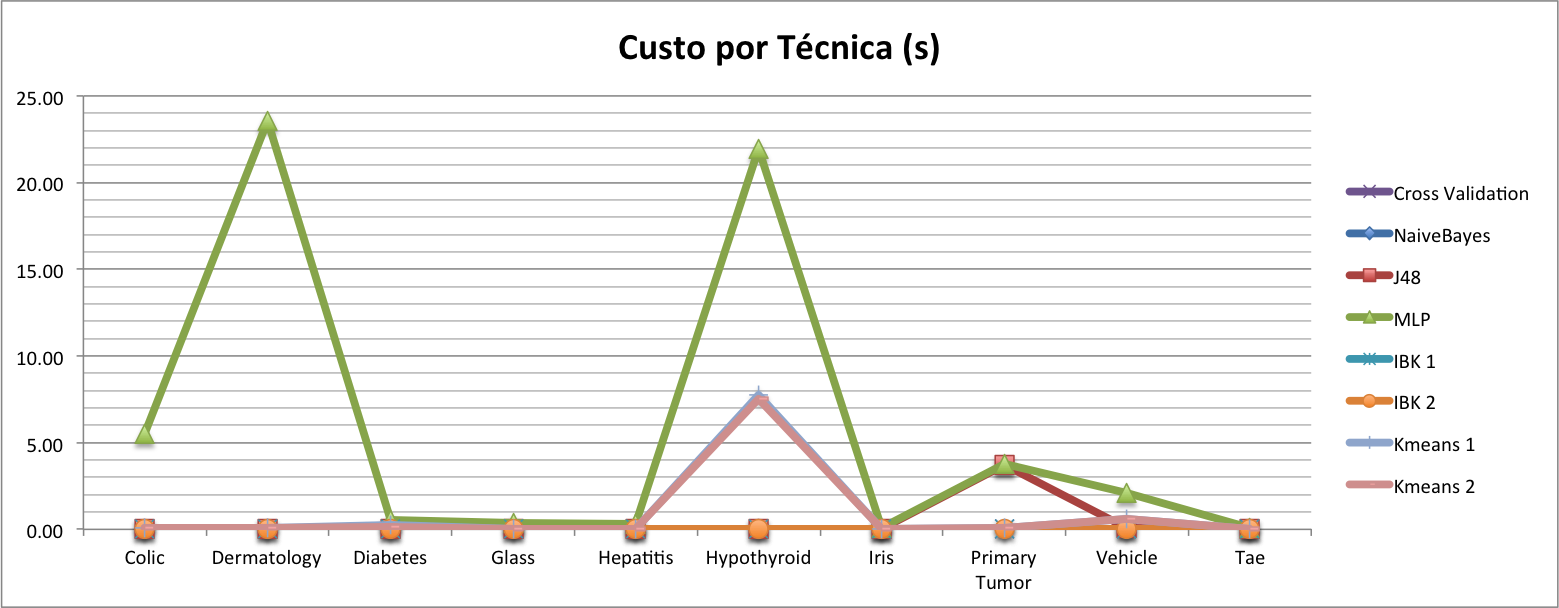
\includegraphics[width=.68\textwidth]{CustoTecnica.png}
\caption{Gráfico do Custo das Técnicas de Aprendizado}
\label{fig:custotecnica}
\end{figure}

A tabela \ref{tabelaCustoConjuntoDados} juntamente com os gráficos da figura \ref{fig:custoconjunto} e figura \ref{fig:custotecnica} mostram que praticamente todas as técnicas são rápidas, exceto MutiLayer Peceptron e kMeans.

\subsection{Split de Dados} \label{sec:splitdados}

Como visto em \ref{sec:split}, foi usado um software para realizar a divisão do conjunto para realização de teste e treinamento. O programa permite selecionar a porcentagem que se deseja para teste e para treinamento. Ao selecionar aleatoriamente, o conjunto é separado de forma aleatória, caso contrário, a divisão é realizada de maneira a coletar-se informações de maneira sequencial.

O conjunto selecionado para estudo do Split deu-se pelo fato de o conjunto apresentar o maior número de amostras, maior acurácia apresentada na tabela \ref{tabelaAcuraciaConjuntoDados} e um dos maiores custos apresentados na tabela \ref{tabelaCustoConjuntoDados}.

Os dados referentes ao split do conjunto de dados \textit{Hypothyroid} estão divididos 80\% para treinamento e 20\% para teste.

A seguir, será mostrado as matrizes de confusão das técnicas J48, NayveBayes, MLP,  e IBk, onde, coincidentemente, as acurácias de treinamento e teste corresponderam a 99,80\% e 99,47\% e o custo das técnicas não extrapolaram 0,04 segundos.

\begin{figure}[!h]
\centering
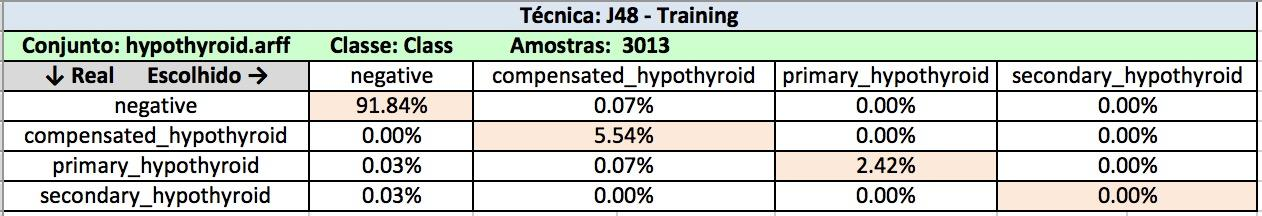
\includegraphics[width=.88\textwidth]{trainj48.png}
\caption{Matriz de Confusão J48}
\label{fig:trainj48}
\end{figure}

\begin{figure}[!h]
\centering
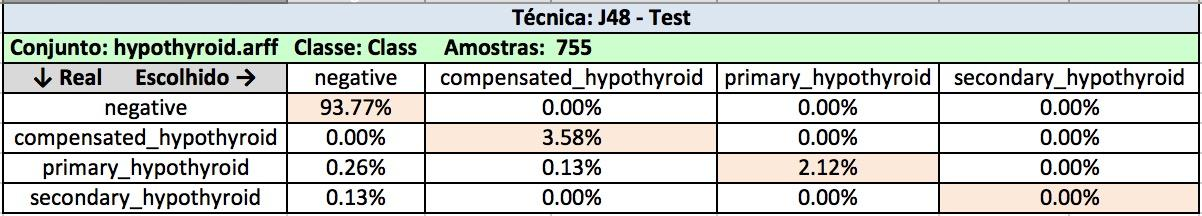
\includegraphics[width=.88\textwidth]{teste-j48.png}
\caption{Matriz de Confusão J48}
\label{fig:testJ48}
\end{figure}

\begin{figure}[!h]
\centering
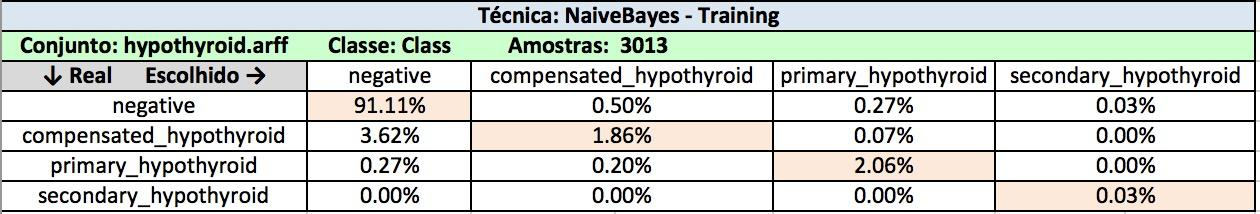
\includegraphics[width=.88\textwidth]{nb-train.png}
\caption{Matriz de Confusão NayveBayes}
\label{fig:trainnb}
\end{figure}

\begin{figure}[!h]
\centering
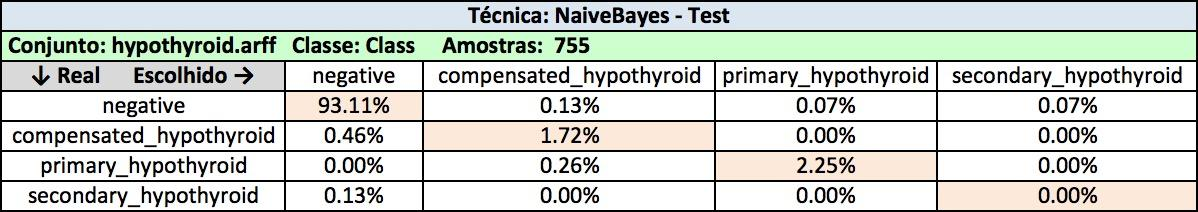
\includegraphics[width=.88\textwidth]{nb-test.png}
\caption{Matriz de Confusão NayveBayes}
\label{fig:testnb}
\end{figure}

\begin{figure}[!h]
\centering
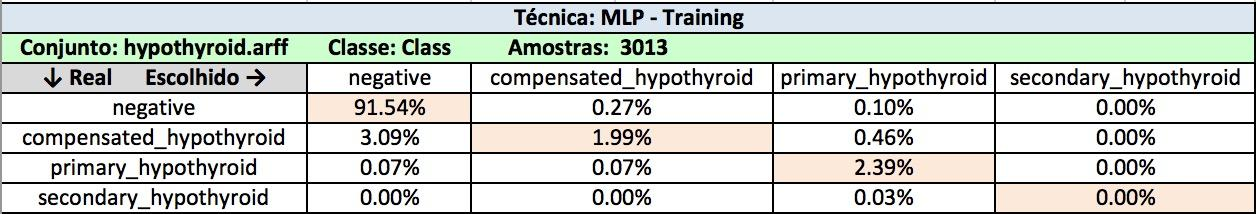
\includegraphics[width=.88\textwidth]{mpl-train.png}
\caption{Matriz de Confusão MLP}
\label{fig:trainmlp}
\end{figure}
\begin{figure}[!h]
\centering
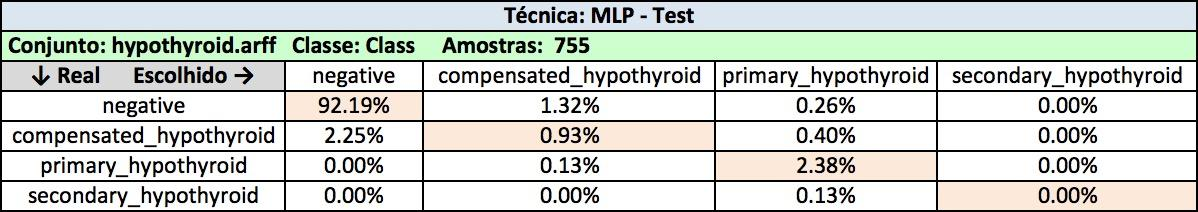
\includegraphics[width=.88\textwidth]{mpl-test.png}
\caption{Matriz de Confusão MLP}
\label{fig:testmlp}
\end{figure}

\begin{figure}[!h]
\centering
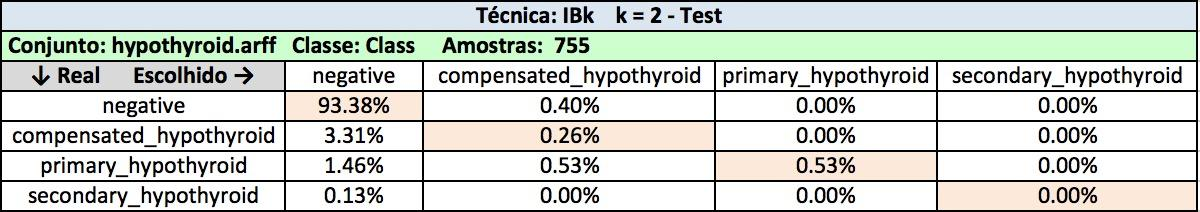
\includegraphics[width=.88\textwidth]{ibk2-train.png}
\caption{Matriz de Confusão IBk = 2}
\label{fig:trainibk2}
\end{figure}

\begin{figure}[!h]
\centering
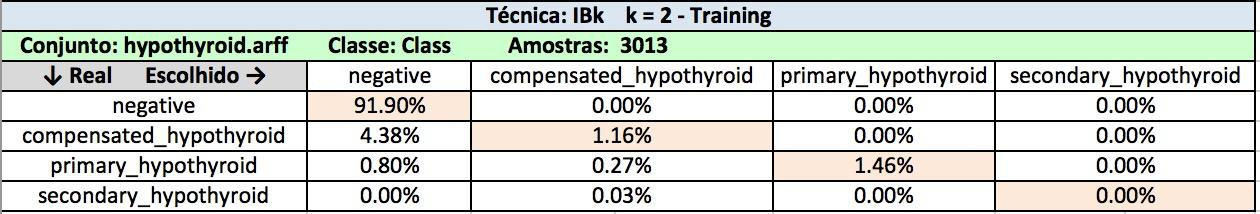
\includegraphics[width=.88\textwidth]{ibk2-test.png}
\caption{Matriz de Confusão IBk = 2}
\label{fig:testibk2}
\end{figure}

\begin{figure}[!h]
\centering
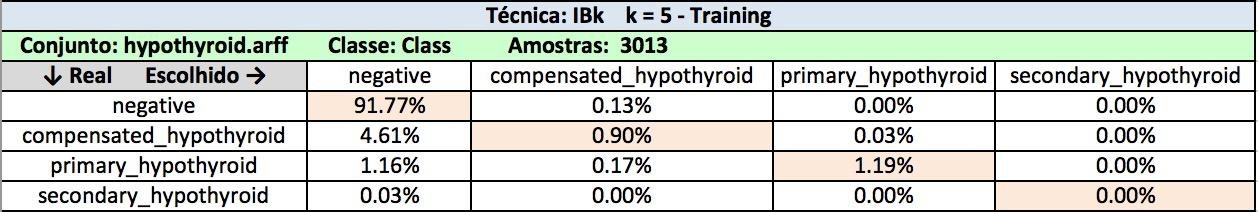
\includegraphics[width=.88\textwidth]{ibk5-train.png}
\caption{Matriz de Confusão IBk = 5}
\label{fig:trainibk5}
\end{figure}

\begin{figure}[!h]
\centering
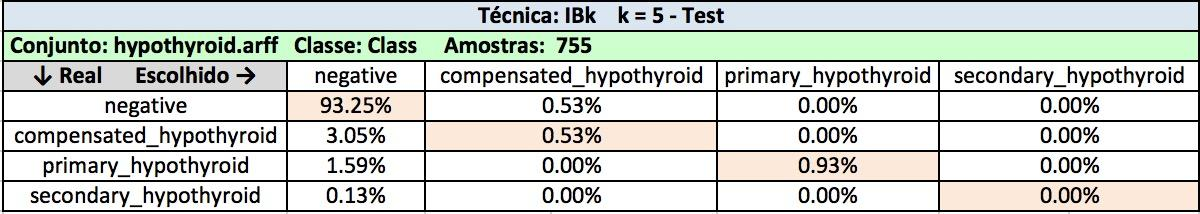
\includegraphics[width=.88\textwidth]{ibk5-test.png}
\caption{Matriz de Confusão IBk = 5}
\label{fig:testibk5}
\end{figure}

%inserindo todas as páginas
%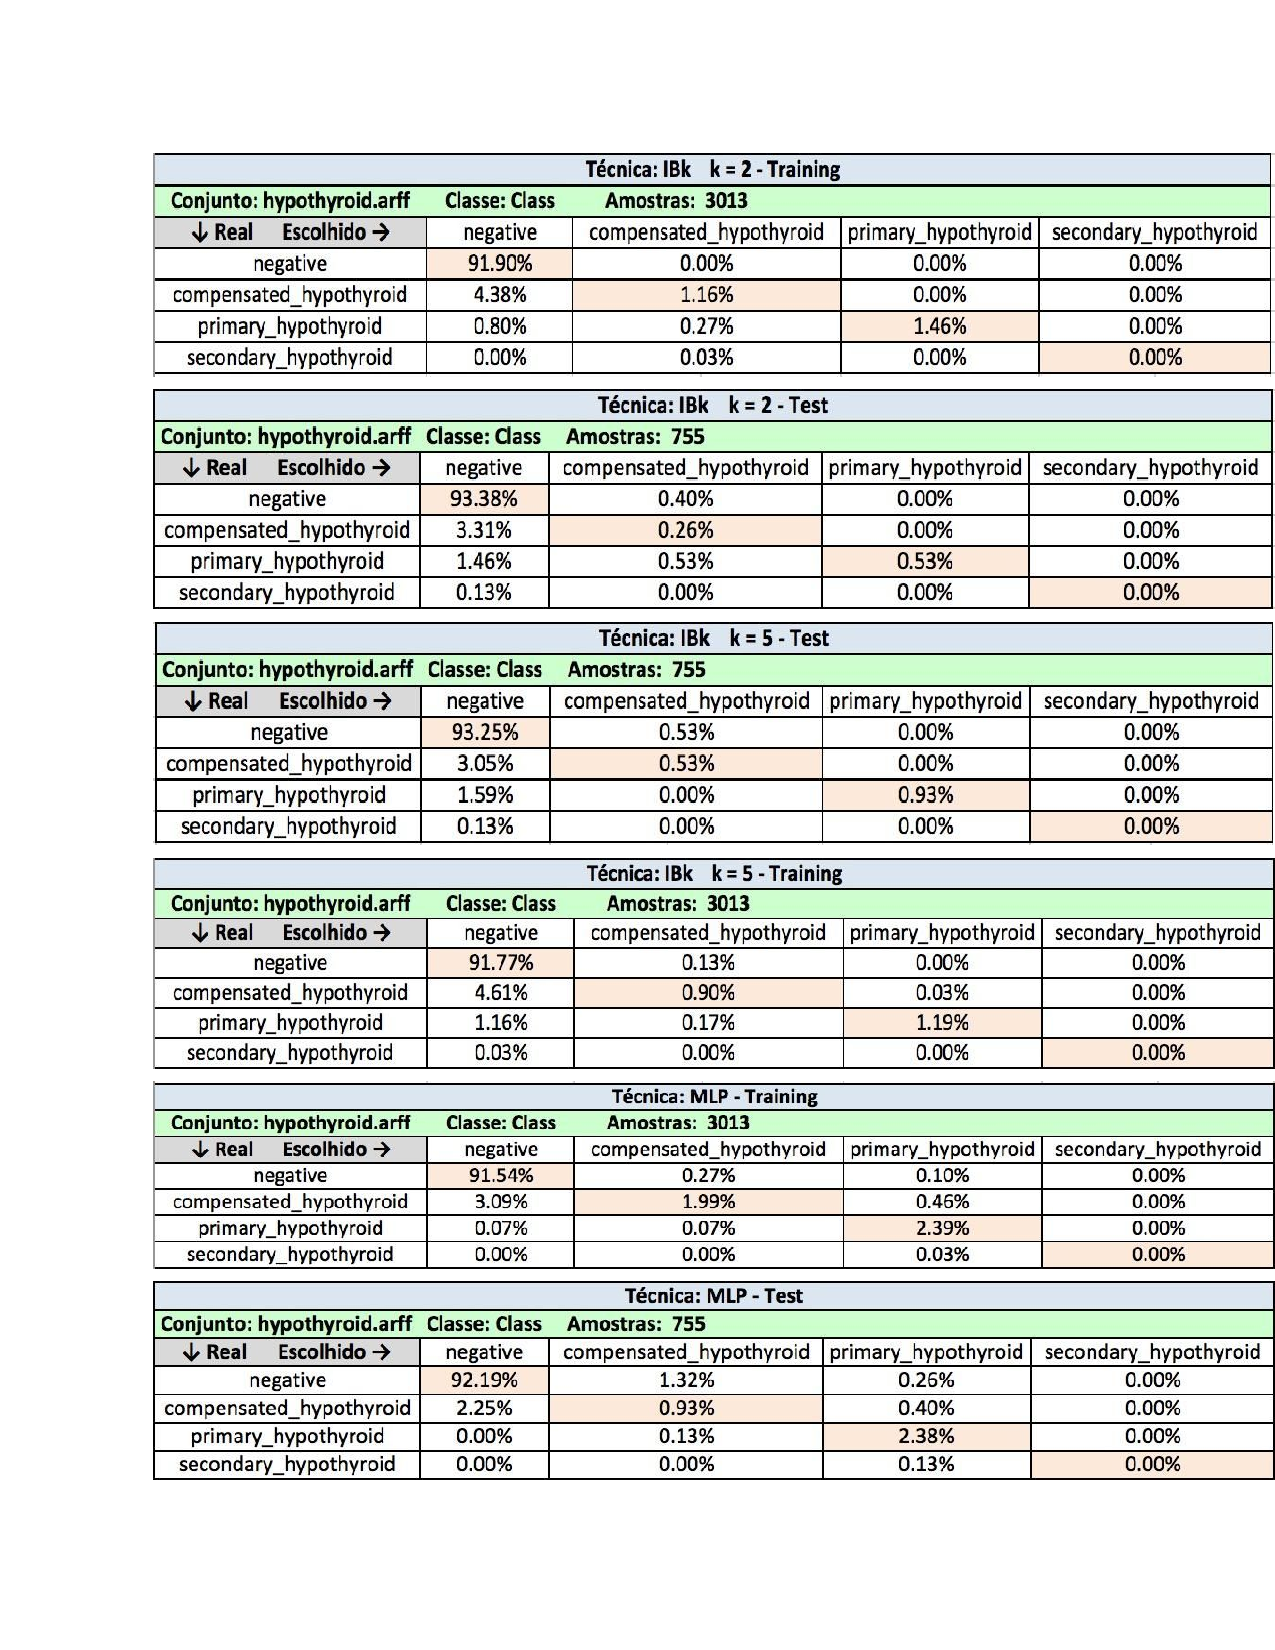
\includepdf[pages=-]{MatrizConfusao.pdf}

\section{Trabalho Correlato} \label{sec:correlato}

Nessa seção será apresentado o trabalho \textit{Lexicographic preferences for predictive modeling of human decision making: A new machine learning method with an application in accounting}\cite{lexic} onde aparece uma nova estratégia de aprendizado.

O algoritmo para expansão dos pares de escolha mais prováveis pode ser visualizado na figura \ref{fig:alglpllr}.
\begin{figure}[h]
	\centering
	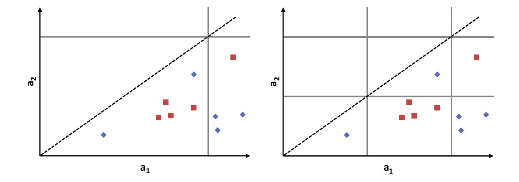
\includegraphics[width=.68\textwidth]{agrupamennto.png}
	\caption{Agrupamento/Expansão dos Atributos de Decisão}
	\label{fig:agrupamento}
\end{figure}

\begin{figure}[h]
	\centering
	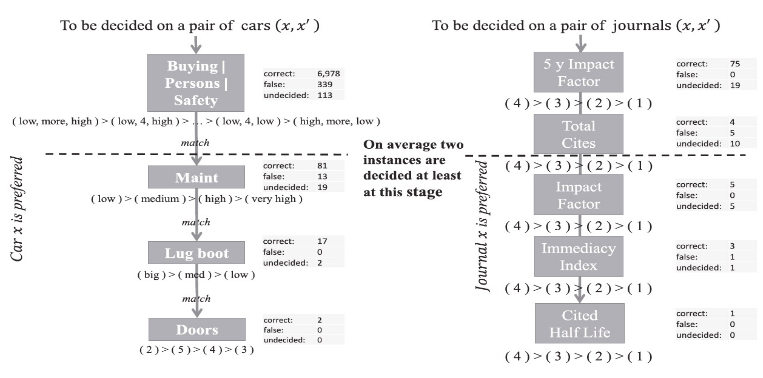
\includegraphics[width=.88\textwidth]{decisao.png}
	\caption{Decisão}
	\label{fig:decisao}
\end{figure}

De acordo com os autores, uma estratégia de tomada de decisão humana é a heurística "Escolher a Melhor", sem integrar todas as informações, apenas de forma "competitiva" escolher a aparentemente melhor.
Outra estratégia é o modelo lexicográfico, que é comparar duas opções, verificando um critério entre eles que difere e usando o mesmo como fator de decisão, sem considerar os demais.

\begin{figure}[h]
	\centering
	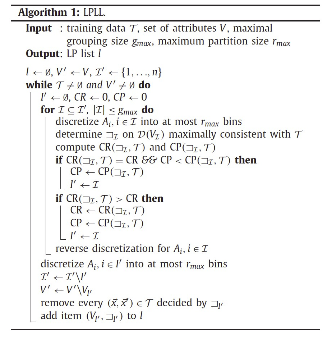
\includegraphics[width=.68\textwidth]{lpll.png}
	\caption{Algoritmo LPLL}
	\label{fig:alglpllr}
\end{figure}

Ao invés de comparar cada atributo separadamente, faz a comparação de todos eles em simultâneo, aproximando-se da heurística humana. Outra diferença proposta pelos autores é um método para discretizar os domínios de atributos numéricos, para análise par a par, facilitando a aplicação da heurística proposta.

Em um estudo de caso, o artigo investiga um problema importante e altamente complexo de decisão do mundo real com relação à elaboração de relatórios financeiros sobre modelo de pensões profissionais (contribuinte/não-contribuinte, segurado/não-segurado, etc.)

Da mesma forma que outras decisões de negócios, a administração da empresa tem que considerar muitos fatores (atributos) ao decidir sobre um método, e pode ser uma boa alternativa aplicar uma heurística lexicográfica.

Possui Lista de Preferências Lexicográficas (LPs) com as alternativas a serem consideradas, onde o algoritmo faz o aprendizado destas listas para, então, tomar as decisões.

 Um exemplo pode ser visto na figura \ref{fig:decisao} onde ocorre a decisão entre um par de carros e um par de artigos, considerando sempre dois atributos.
 
 O Agrupamento dos atributos de decisão pode ser observado na figura \ref{fig:agrupamento} onde à esquerda existe apenas uma divisão e, na direita, duas divisões, onde cada divisão possui elementos "puros", sendo eles do tipo vermelho (negativo) ou do tipo azul (positivo).
 
\begin{equation}
\centering
x\in\mathbb{X}={D(V)}={D(A_1)}\times{...}\times{D(A_n)}
\end{equation}

Onde V são as alternativas e D os domínios dos atributos.
\begin{equation}
\centering
\tau={(x_1^{*},x_i)}_{(i=1)}^{N}
\end{equation}

\section{Conclusão} \label{sec:conclusao}

O estudo permitiu verificar que o aprendizado supervisionado possui maior acurácia, por terem especificadas as classes, assim como observar que o aprendizado não-supervisionado é melhor quando não se há muita informação a respeito do conjunto de dados a ser analisado.

Após empregar aa divisão para treinamento e teste dos conjuntos de dados, todas as técnincas obtiveram resultados superiores a 90\%, ou seja, aumento de precicisão nos dados e maior confiabilidade.

Mais atributos/dimensões resultam numa melhor classificação, porém deve-se atentar à maneira com que seleciona-se tais dados. Técnicas de aprendizado ativo não foram citadas, mas podem fazer muita diferença quando os conjuntos de dados são muito grandes.

Se o conjunto de dados é muito grande, o computador que está executando o experimento deve conter muita memória RAM! As técnicas de aprendizado facilitam na quantidade das classificações, mas têm um grande custo computacional.

\bibliographystyle{sbc}
\bibliography{sbc-template}


\end{document}
